El detector de símbolos necesario para lograr una prueba de funcionamiento de los circuitos integrados compuestos por el front-end analógico de un sistema RFID, se desarrolló mediante el lenguaje de descripción de hardware (HDL) Verilog.

\subsection{Características de la comunicación}

\subsubsection{Frames}
La ISO/IEC14443 tipo A agrupa los bits de datos en un frame con un comienzo de frame (SoF), un fin de frame (EoF) y un bit de paridad (P) al final de cada byte de datos (8 bits de datos), excepto para frames cortos. El EoF solo se usa para la comunicación desde el PCD a PICC.

\begin{figure}[H]
\centering
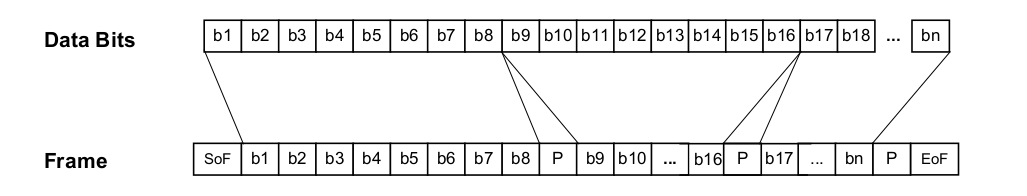
\includegraphics[scale=0.5]{digital/Frame_TipoA.png}
\caption{Formato de frame de Tipo A.}
\label{fig:frame_A}
\end{figure}

\subsubsection{Codificaciones}
Debido a la dificultad para determinar la diferencia entre un bit cero y el transmisor realmente desconectado, los datos necesita algunas reglas adicionales, es decir, debe codificarse. Los métodos de codificación utilizados en esta especificación son:

\begin{itemize}
\item Manchester \ref{fig:coding_A}.
\item Miller modificado \ref{fig:coding_A}.
\end{itemize}

\begin{figure}[H]
\centering
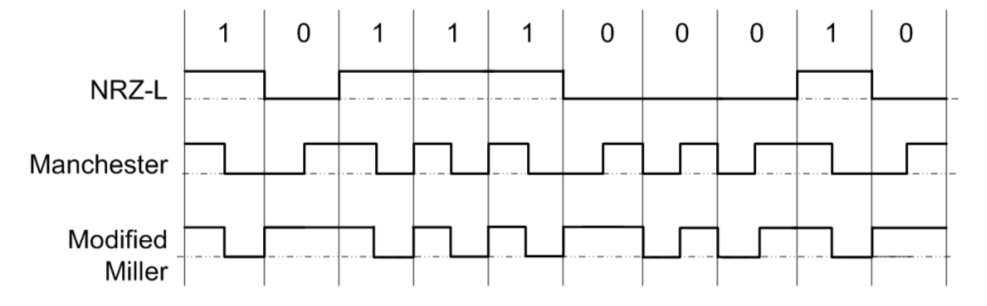
\includegraphics[scale=0.5]{digital/Codificaciones.png}
\caption{Codificaciones utilizadas.}
\label{fig:coding_A}
\end{figure}

En la Tipo A se utiliza la codificación Manchester para la comunicación del PICC hacia el PCD y Miller Modificado para la del PCD hacia el PICC.

\subsubsection{Bit Rate}
El tiempo de una señal digital se indica por medio de unidades de tiempo elementales (etu).
Para esta especificación, un etu equivale a un período de un bit, es decir, el tiempo para transmitir una unidad de información.\newline
Para la comunicación PCD -> PICC:
$$ 1 etu =  \frac{128}{f_c D_{PCD->PICC}}$$\newline
Para la comunicación PICC -> PCD:
$$ 1 etu =  \frac{8}{f_s D_{PICC->PCD}}$$
Donde $f_c$ es la frecuencia de portadora generada por el PCD, $f_s$ la frecuencia de subportadora generada por el PICC. El valor inicial de los dividores $D_{PCD->PICC}$ y $D_{PICC->PCD}$ es 1, lo que da una velocidad de bit inicial de 106kb/s.
Entonces, durante este documento, se hablará de una velocidad de bit de $f_c$/128 \~ 106kbit/s en ambas direcciones de la comunicación.


\subsubsection{Sincronización}
A diferencia de la Tipo B, la Tipo A no tiene una secuencia de sincronización. Para la comunicación desde el PCD al PICC, la Tipo A usa 100\% ASK. El nivel inferior es un disparador suficiente para iniciar la demodulación e indicar el inicio del primer símbolo.
Para la comunicación PICC a PCD, la comunicación es síncrona y alineada a la cuadrícula. El inicio de una secuencia se determina contando el número de ciclos de la portadora transcurridos desde el último nivel inferior del comando.

\subsubsection{Codificación de bits}
Aquí se especifica cómo son los valores lógicos para la norma ISO/IEC14443 Tipo A.

La codificación utilizada por el PCD es Miller Modificado con modulación ASK 100\% (Fig. \ref{fig:Mil}).

\begin{figure}[H]
\centering
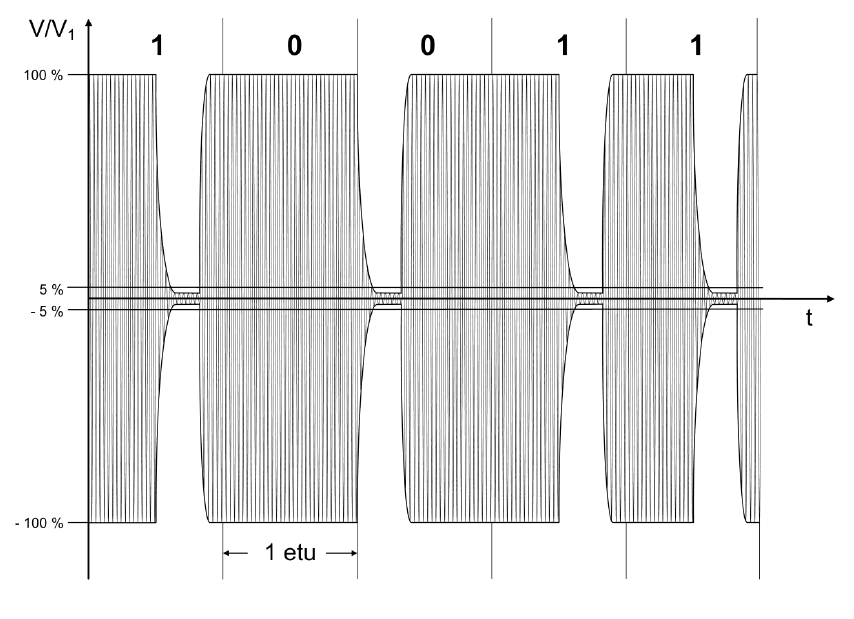
\includegraphics[scale=0.5]{digital/Miller_Modif.png}
\caption{Miller modificado con modulación ASK al 100\%.}
\label{fig:Mil}
\end{figure}

Los símbolos definidos son los siguientes:
\begin{itemize}
\item Símbolo X: nivel bajo luego de la mitad de la duración del bit.
\item Símbolo Y: toda la duración del bit sin modulación.
\item Símbolo Z: el comienzo del bit en nivel bajo.
\end{itemize}

La codificación utilizada por el PICC es Manchester con modulación OOK con subportadora (Fig. \ref{fig:Man}).

\begin{figure}[H]
\centering
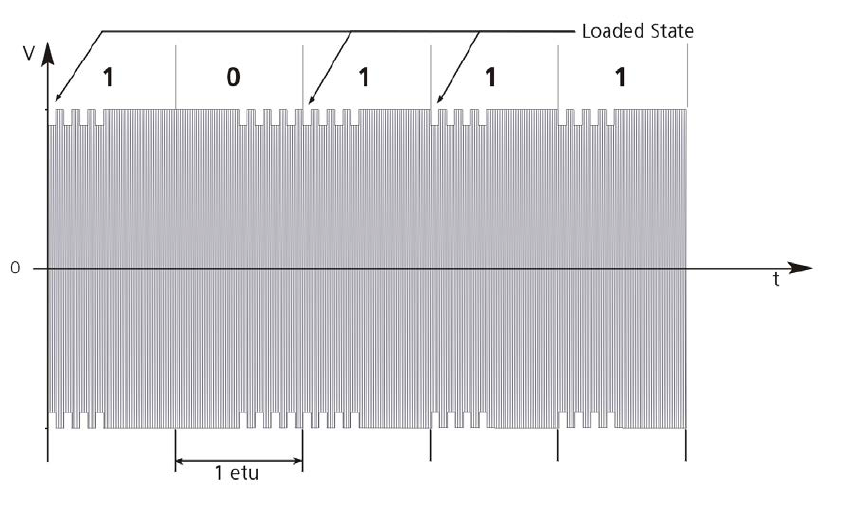
\includegraphics[scale=0.5]{digital/Manchester.png}
\caption{Codificación manchester con modulación OOK.}
\label{fig:Man}
\end{figure}

Los símbolos definidos son los siguientes:
\begin{itemize}
\item Símbolo D: la portadora es modulada por la subportadora durante la primer parte del bit.
\item Símbolo E: la portadora es modulada por la subportadora durante la segunda parte del bit.
\item Símbolo F: la portadora no es modulada por la subportadora durante toda la duración del bit.
\end{itemize}

\subsubsection{Desincronización}
Consiste en una violación de las reglas normales de codificación/decodificación para un "0" lógico y un "1" lógico.


\subsubsection{Formato de frame}
En esta sección se definen los frames utilizados en la norma tipo A. 
Ésta utiliza dos tipos de frames:
\begin{itemize}
\item Frame corto.\\
El frame corto es utilizado para comenzar la comunicación y consiste en lo siguiente (Fig.\ref{fig:short_frame}):\\
- SoF ( Inicio de trama - Start of frame ).\\
- 7 bit de información transmitidos primero los LBS.\\
- EoF ( Fin de trama - End of Frame ).\\
No se añade paridad.
\end{itemize}

\begin{figure}[H]
\centering
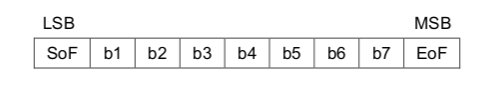
\includegraphics[scale=0.5]{digital/Short_Frame.png}
\caption{Frame corto.}
\label{fig:short_frame}
\end{figure}

\begin{itemize}
\item Frame standar.\\
 El frame standar para el intercambio de información y consiste en lo siguiente (Fig\ref{fig:standar_frame}).\\
 - SoF.\\
 - n x (8 bits de información + bit de paridad impar), con n \geq  1.\\
 - EoF (sólo desde el PCD al PICC).
\end{itemize}

\begin{figure}[H]
\centering
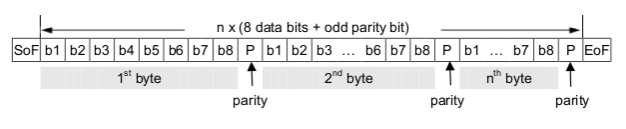
\includegraphics[scale=0.5]{digital/Standar_Frame.png}
\caption{Frame standar.}
\label{fig:standar_frame}
\end{figure}

Para la comunicación desde el PCD al PICC, el SoF debe ser un "0" lógico.
Para la comunicación desde el PICC al PCD, el SoF debe ser un "1" lógico.
Para la comunicación PCD a PICC, un frame debe terminar con EoF.
Este EoF debe ser un "0" lógico.

\subsubsection{Tamaños de frame}
\begin{itemize}
\item FSD (Tamaño de frame para el PCD).\\
El FSD define el tamaño máximo de un frame que el PCD es capaz de recibir. El FSD es expresado en número de bytes de datos incluidos en el frame.\\ 
Para el Tipo A, el PCD
indica el FSD al PICC por el parámetro FSDI con el comando RATS 
\item FSC (Tamaño de frame para el PICC).\\
El FSC define el tamaño máximo de un frame aceptado por el PICC. El FSC es expresado en número de bytes de datos incluidos en el frame.\\ 
Para el tipo A, el PICC
indica el FSC a PCD por medio del FSCI en T0 del comando ATS.
\end{itemize}


\subsubsection{Set de comandos}

\begin{table}[H]
\centering
\begin{tabular}{c|c|c|c}
\textbf{Comando PCD} & \textbf{Respuesta PICC}                                                   \\ \hline
WUPA                    & ATQA                                                                        \\
REQA                 	& ATQA                                                                         \\
ANTICOLLISION CL1                  & UID CL1                                                                             \\
ANTICOLLISION CL2                  & UID CL2                                                                            \\
ANTICOLLISION CL3                 & UID CL3                                                                             \\
SELECT CL1                  & SAK                                                                            \\
SELECT CL2                  & SAK                                                                          \\
SELECT CL3                  & SAK                                                                                 \\
HLTA                  & -                                                                           \\
RATS                  & ATS       
\end{tabular}
\caption{Set de comandos}
\label{table:set_com}
\end{table}

\subsection{Estructura general del detector}
En la figura \ref{fig:dig_diag} se observa la estructura del detector de símbolos realizado.
Este detector consta de dos etapas de "traducción" de datos: un decodificador para convertir la información codificada por el PCD con Miller Modificado y un codificador para convertir la información generada por el PICC con codificación NRZ-L a codificación Manchester. Además, 

\begin{figure}[H]
\centering
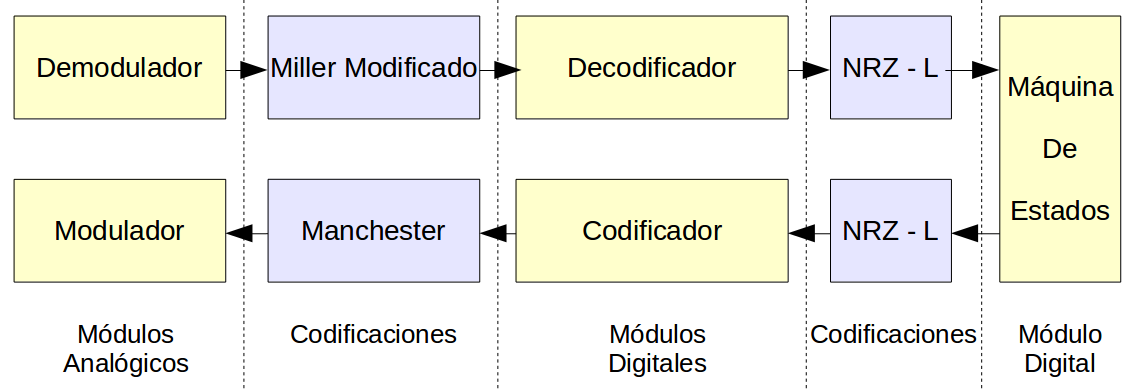
\includegraphics[scale=0.3]{digital/Diagrama_Digi.png}
\caption{Diagrama básico del detector de símbolos.}
\label{fig:dig_diag}
\end{figure}

\subsection{Codificador}
Como ya se mencionó y, además, como puede observarse en la figura \ref{fig:dig_diag}, el codificador es el encargado de tomar los datos que genera la máquina de estado en NRZ-L y convertirlos en codificación Manchester para que ingresen al modulador de carga, transmitiendo, así, el mensaje desde el PICC al PCD.
El módulo responde a lo visto en la figura \ref{fig:Man}:
\begin{itemize}
\item Modula la portadora con la subportadora durante la primer mitad del bit cuando a su entrada llega un "1" lógico.
\item Modula la portadora con la subportadora durante la segunda mitad del bit cuando a su entrada llega un "0" lógico.
\end{itemize}
En la imagen \ref{fig:manch_code} se observa el módulo descripto mediante el lenguaje Verilog.

\begin{figure}[H]
\centering
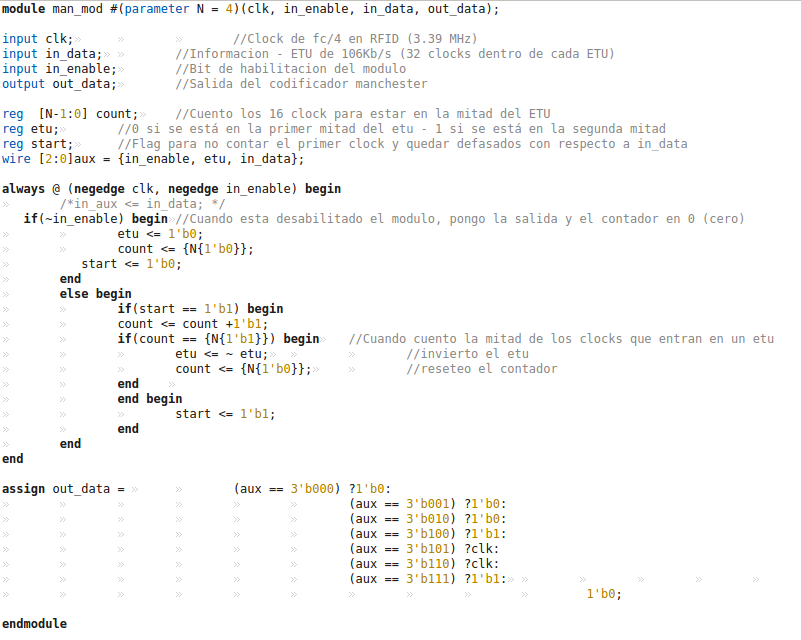
\includegraphics[scale=0.45]{digital/Manchester_code.png}
\caption{Codificador Manchester en Verilog.}
\label{fig:manch_code}
\end{figure}

Durante el desarrollo de los módulos digitales del proyecto, se utilizó el "Icarus Verilog", una herramienta de compilación, síntesis y simulación de Verilog (IEEE-1364). Además del compilador mencionado, se usó el software para visualización de señales "GtkWave".
En la figura \ref{fig:manch_test} se muestra el resultado del testbench del módulo codificador con el GtkWave como herramienta de visualización de señales.

\begin{figure}[H]
\centering
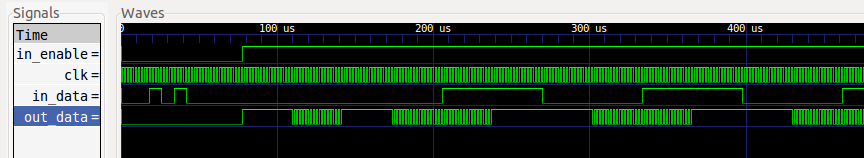
\includegraphics[scale=0.5]{digital/Manchester_testbench.png}
\caption{Testbench del codificador Manchester.}
\label{fig:manch_test}
\end{figure}

En la etapa en la que el PICC debe comunicarse con el PCD, siempre habrá portadora, por esto es que se observa una señal de clock constante. Cada módulo contiene tanto un PoR (Power on Reset) que activa toda la lógica cuando el chip se energiza y una señal de habilitación (in\_ enable) que forma parte de la lógica de habilitación y desabilitación de los módulos durante la comunicación.
Una vez que la señal de habilitación se encuentra en estado alto, puede observarse que el codificador comienza a trabajar.

\subsection{Decodificador}

El módulo decodificador recibe las señales enviadas en codificación Miller Modificado por el PCD y demoduladas en el PICC para convertirlas a codificación NRZ-L, lo cuál ingresará a la máquina de estados como bits, puramente, en nivel alto ("1" lógicos) y bits, puramente, en nivel bajo ("0" lógicos). El conexionado de estas etapas puede observarse en la figura \ref{fig:dig_diag}.
En este caso, a diferencia del caso del codificador mencionado antes, la señal de clock, no es constante. Esto trae como necesidad la adición de un detector de pausa dentro del mismo decodificador, ya que al no tener clock, la lógica secuencial se ve afectada. Tanto el clock discontínuo (in\_ clock), como la señal del detector de pausa (in\_ pause) y las respectivas entradas y salidad de datos pueden observarse en la figura \ref{fig:mill_test}.

\begin{figure}[H]
\centering
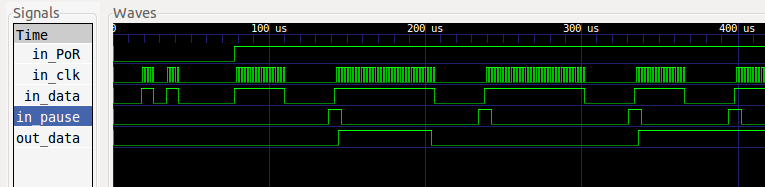
\includegraphics[scale=0.5]{digital/Miller_testbench.png}
\caption{Testbench del decodificador Miller Modificado.}
\label{fig:mill_test}
\end{figure}

\subsection{Detección de los símbolos}
Los datos de salida del módulo decodificador ingresan en codificación NRZ-L a la máquina de estados. Esta máquina funciona siguiendo la lógica mostrada en la sección sobre la "Clasificación y estandarización de los sistemas RFID" donde se muestra en detalle lo normalizado por la norma ISO/IEC 14443 Tipo A.
En el desarrollo, se llevó a cabo la detección del comando REQA enviado por el PDC, respondiendo, una vez detectado, el comando ATQA. Puede observarse el resultado, obtenido en el banco de prueba, en la sección \ref{sec:resmedver}.
